\documentclass{article}
\usepackage{amsmath}
\usepackage{graphicx}
\usepackage{listings}
\usepackage{hyperref}
\usepackage{booktabs}
\usepackage{xcolor}
\usepackage{geometry}
\usepackage{multicol}

\geometry{a4paper, margin=1in}

\title{Lumina: Revolutionizing Academic Search}
\author{
    Ishaan Kapoor \\
    \texttt{ishaan@lumina-chat.com} \\
    \and
    Mehul Chadda \\
    \texttt{mehul@lumina-chat.com} \\
    \and
    Akhilesh Sharma \\
    \texttt{akhilesh@lumina-chat.com}
}
\date{}

\begin{document}

\maketitle
\begin{abstract}
    Every month, fifty million researchers use Google Scholar to find and validate research for projects, grants, and more. Advances in computing, embedding models, and transformer models can revolutionize this process. Our new search solution, Lumina, leverages these technologies to be 100 times more effective than traditional methods like Google Scholar and Semantic Scholar at finding the most relevant research. Lumina searches over 2 billion vectors and 2 trillion tokens, in milliseconds and outperforms leading search APIs zero-shot.
    Lumina shows you pinpointed sections within a relevant paper, benchmarking highest at context precision, avoiding over-summarization and providing precise information to make skimming faster. We benchmarked Lumina's search results against Google Scholar, Semantic Scholar, and Exa measuring the Context Precision, and Context Relevance of each search result, observing an X\% improvement across the board. By employing novel ingestion pipelines, search infrastructure, and search evaluation tools, Lumina sets a new standard for precision and utility in academic research. The benchmark code and datasets are public, establishing a baseline for future comparisons.
\end{abstract}

\newpage

\begin{multicols}{2}

\section{Overview}
Search for academic research often suffers from poor tooling, leading to countless hours wasted finding and validating information. Most solutions today attempt to mitigate this by either employing slow and expensive large language model chains (LLMs) or by attempting to do semantic search. However, these solutions only address symptoms of the underlying issue, resulting in slow and/or inaccurate searches. LLM chains are slow, expensive, and need extensive context to perform well, and existing semantic search solutions like Semantic Scholar API, have poor search results despite having a detailed and well maintained corpus. The core problem lies in the inadequacy of current search infrastructure, which fails to return high-quality, relevant results efficiently.

\section{Background}
We introduce Lumina, the top-performing search engine and API for academic research, leading benchmarks in both context relevance (how accurate our search is) and context precision (the signal-to-noise ratio of our results). 
Lumina has 2 distinct advantages to other search datasets. Firstly, we have a very robust ingestion pipeline, that extracts figure content, formula content, in text references and citation trials and indexes them all. We also intelligently create a series of embeddings for each paper and combine advantage of many different search solutions (semantic, fulltext and AI) allowing us to cater to both quick (broad) searches and deep dives (specific).
We benchmarked on two datasets: 10,000 LLM generated research questions and 10,000 open-source real user queries from the SciSpace platform. Lumina consistently outperforms other search systems, providing highly relevant and precise results across various scenarios.

\subsection{Lumina Search Infrastructure}

\subsubection{Data}
Open alex
Arxiv dump
Used LLMs to extract metadata
\section{Methodology}
We developed a comprehensive benchmark that processes a large number of questions through multiple search providers. For each question, the system retrieves search results from each provider, processes the content, and evaluates the relevance and precision of the retrieved information using GPT-4o as a judge. We compare the search results from different providers based on two primary metrics: context relevance and context precision. These metrics are calculated for each search result and then aggregated to provide an overall performance score for each provider.
\begin{figure}[h]
    \centering
    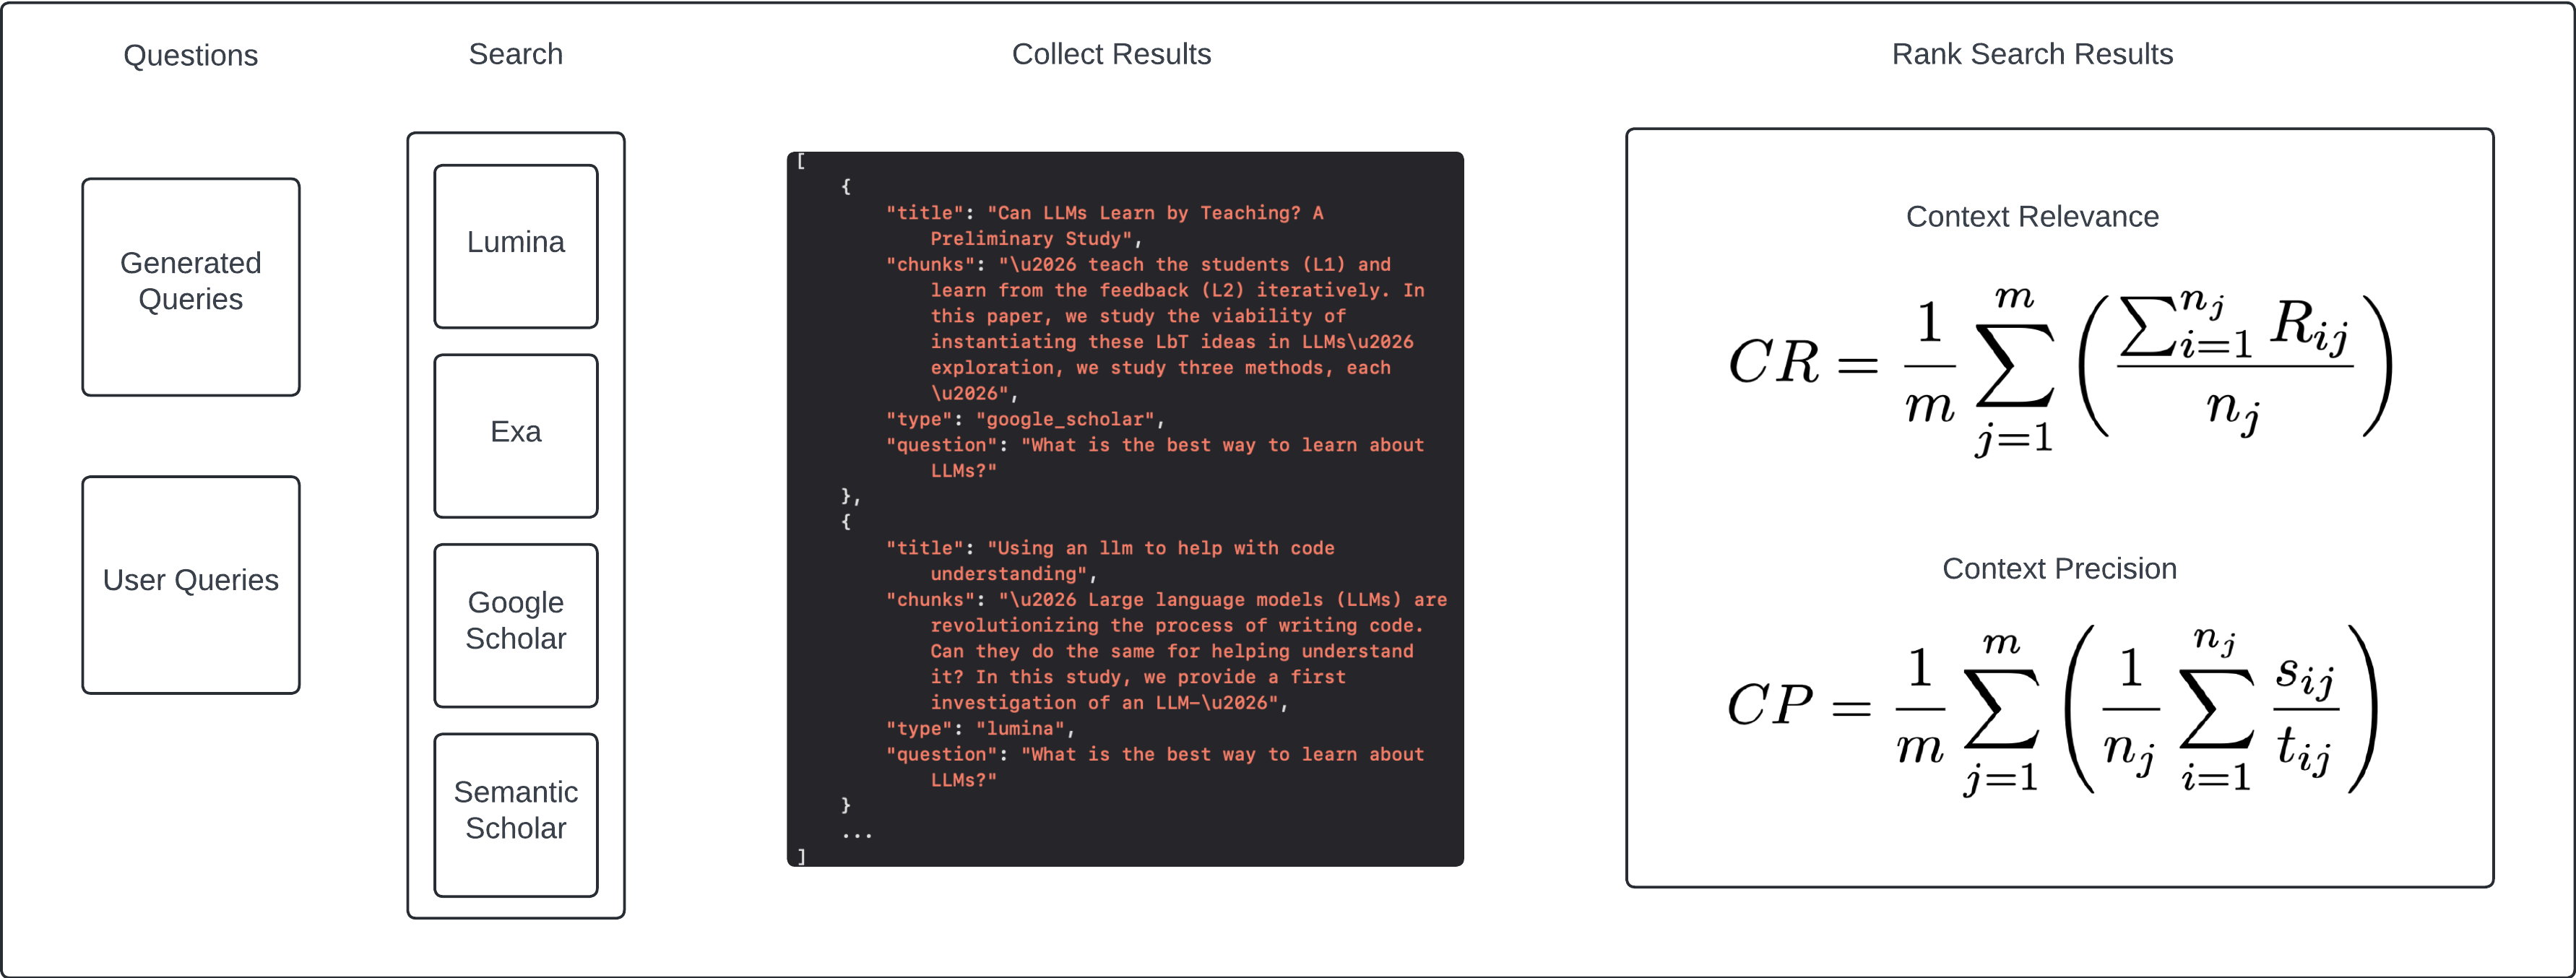
\includegraphics[width=\columnwidth]{Benchmark_Overview_main.png}
    \caption{Benchmark System Workflow}
\end{figure}
The benchmark evaluates the following search providers:
\begin{description}
    \item[Semantic Scholar:] A popular semantic research tool for scientific literature. Accessed via Semantic Scholar's API.
    \item[Google Scholar:] A freely accessible web search engine that indexes the full text or metadata of scholarly literature. Accessed via SERP API.
    \item[Exa:] Exa.ai is an AI-powered search engine that aims to provide more advanced and semantic search capabilities compared to traditional search engines. Accessed via Exa's API.
    \item[Lumina:] Our new search solution leveraging advanced technologies for superior search performance. Accessed via Lumina's API.
\end{description}
\subsection{Datasets}
Two distinct datasets are used in this benchmark, each serving a unique purpose in our evaluation process. By utilizing both synthetic and real-world queries, we aim to provide a comprehensive and balanced assessment of search provider performance across various scenarios. This dual-dataset approach allows us to test both the theoretical capabilities and practical effectiveness of each search engine in academic contexts. The datasets are as follows:

\begin{itemize}
    \item \textbf{Synthetically Generated Questions:} 10,000 questions generated using Claude's Sonnet, covering a wide range of academic topics and complexities.
    \item \textbf{User Queries from SciSpace:} We collected 10,000 real user queries, hosted openly on the SciSpace platform, representing actual research questions posed by academics and researchers. This dataset is a good proxy for "real world" questions inputted into a search bar.
\end{itemize}

\subsection{Metrics}
A search result consists of a question and its corresponding contexts. For each question, we call the search route for each API and collect the results. We then iterate through these contexts to calculate the metrics per question per provider.

\subsubsection{Context Relevancy (CR)}
This metric evaluates the proportion of relevant contexts among the total contexts retrieved for a query. For each search result, GPT-4o acts as a judge and determines if each context is relevant or not using the Context Relevance Prompt (Appendix~\ref{sec:context_relevance_prompt}). The relevancy scores for all search results are then averaged to get the overall CR for each search provider.
\begin{equation}
CR = \frac{1}{m} \sum_{j=1}^{m} \left( \frac{\sum_{i=1}^{n_j} R_{ij}}{n_j} \right)
\end{equation}
Where:
\begin{itemize}
    \item $m$ is the total number of search results
    \item $n_j$ is the total number of contexts in search result $j$
    \item $R_{ij}$ is a binary relevance indicator (1 if relevant, 0 if not) for context $i$ in search result $j$. This is determined by GPT-4o using the Context Relevance Prompt (Appendix~\ref{sec:context_relevance_prompt}).
\end{itemize}

\subsubsection{Context Precision (CP)}
This metric evaluates the precision of the relevant information within each context. For each search result, GPT-4o acts as a judge and evaluates each sentence within a context to determine if it is critical or not using the Context Precision Prompt (Appendix~\ref{sec:context_precision_prompt}). The precision scores for all search results are then averaged to get the overall CP for each search provider.
\begin{equation}
CP = \frac{1}{m} \sum_{j=1}^{m} \left( \frac{1}{n_j} \sum_{i=1}^{n_j} \frac{s_{ij}}{t_{ij}} \right)
\end{equation}
Where:
\begin{itemize}
    \item $m$ is the total number of search results
    \item $n_j$ is the total number of contexts in search result $j$
    \item $s_{ij}$ is the number of relevant sentences in context $i$ in search result $j$. This is determined by GPT-4o using the Context Precision Prompt (Appendix~\ref{sec:context_precision_prompt}).
\end{itemize}

We will also implement a recursive search algorithm for each provider, using initial search results to generate more specific, refined queries. This process will be repeated for a set number of iterations (depths) and with varying page sizes. The performance will be evaluated across different combinations of recursion depths and page sizes to understand how these parameters affect search quality.

\section{Results}

\subsection{Context Relevancy}
\subsubsection{Zero-Shot}
Figure~\ref{fig:search_results_zeroshot} shows the average Context Relevancy (CR) scores for different search providers. The CR metric evaluates the proportion of relevant contexts among the total contexts retrieved for a query.

\begin{figure}[h]
    \centering
    \includegraphics[width=0.45\columnwidth]{search_results.png}
    \caption{Context Relevancy Scores by Search Engine and LLM (Zero-Shot)}
    \label{fig:search_results_zeroshot}
\end{figure}

Lumina achieved \textbf{300\%} context relevancy compared to Google Scholar and Semantic Scholar, despite having a smaller search domain (100M vs 200M vs 300M). The graph evaluates performance against both synthetically generated questions and real user queries from SciSpace. 

\subsubsection{Recursive}

Figure~\ref{fig:search_results_recursive} shows the average Context Relevancy (CR) scores for different search providers. The CR metric evaluates the proportion of relevant contexts among the total contexts retrieved for a query.

\begin{figure}[h]
    \centering
    \includegraphics[width=0.45\columnwidth]{search_results.png}
    \caption{Context Relevancy Scores by Search Engine and LLM (Recursive)}
    \label{fig:search_results_recursive}
\end{figure}

Lumina achieved \textbf{300\%} context relevancy compared to Google Scholar and Semantic Scholar, despite having a smaller search domain (100M vs 200M vs 300M). The graph evaluates performance against both synthetically generated questions and real user queries from SciSpace. 

\subsection{Context Precision}
\subsubsection{Zero-Shot}

Figure~\ref{fig:recursive_results_zeroshot} shows the average Context Precision (CP) scores for different search providers. The CP metric evaluates the precision of the relevant information within each context.

\begin{figure}[h]
    \centering
    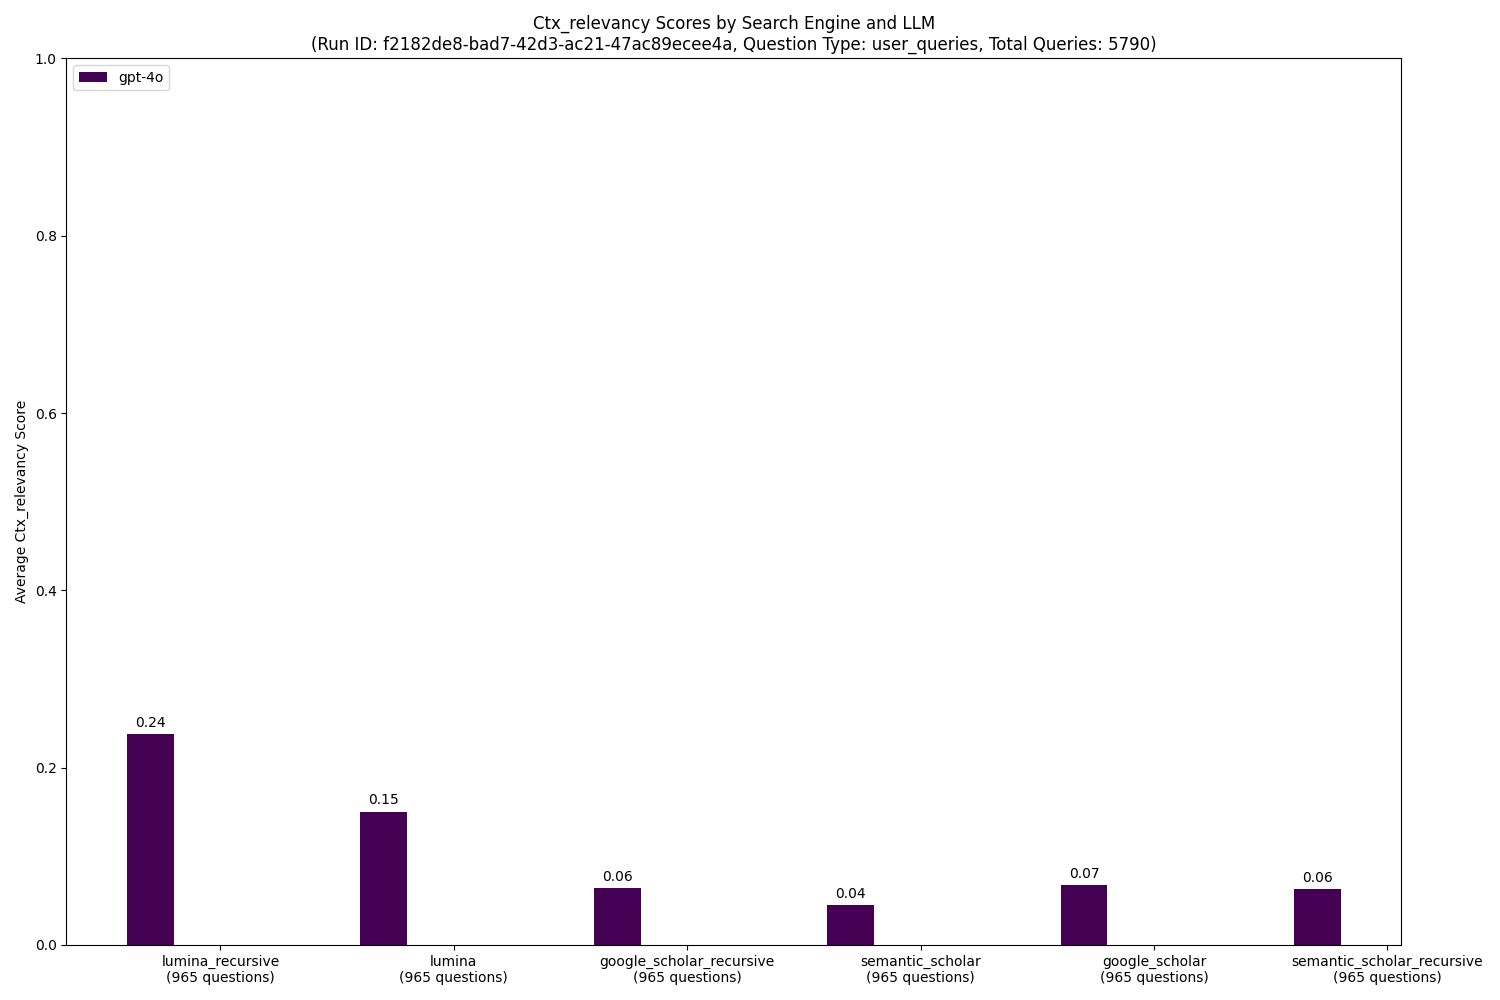
\includegraphics[width=0.45\columnwidth]{recursive_results.png}
    \caption{Context Precision Scores by Search Engine and LLM (Zero-Shot)}
    \label{fig:recursive_results_zeroshot}
\end{figure}

\subsubsection{Recursive}
Figure~\ref{fig:recursive_results_recursive} shows the average Context Precision (CP) scores for different search providers. The CP metric evaluates the precision of the relevant information within each context.

\begin{figure}[h]
    \centering
    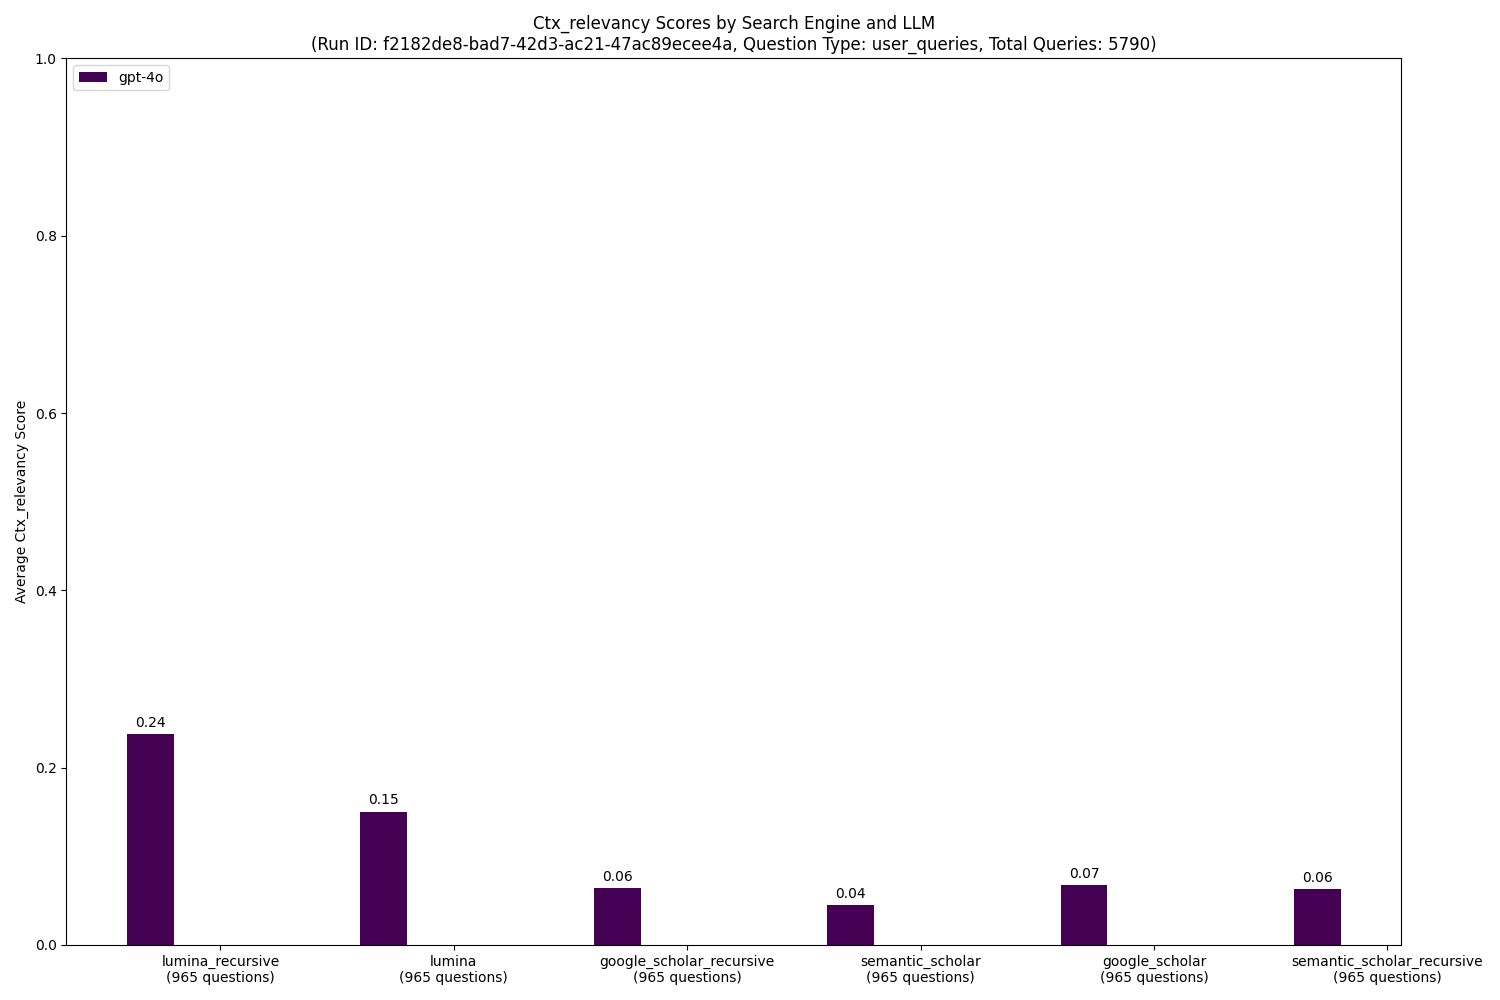
\includegraphics[width=0.45\columnwidth]{recursive_results.png}
    \caption{Context Precision Scores by Search Engine and LLM (Recursive)}
    \label{fig:recursive_results_recursive}
\end{figure}


\subsection{Interpretation of Results}
The results indicate that Lumina significantly outperforms other search providers in both Context Relevancy and Context Precision metrics. Specifically, Lumina's recursive search method achieves the highest CR score of 0.24, compared to 0.15 for its non-recursive counterpart. This demonstrates the effectiveness of Lumina's recursive search in retrieving highly relevant contexts.

In comparison, other search providers such as Google Scholar and Semantic Scholar, both in their standard and recursive forms, achieve much lower CR scores, with the highest being 0.07 for Google Scholar. This highlights Lumina's superior ability to find relevant research objects quickly and accurately.

Similarly, in terms of Context Precision, Lumina again outperforms other providers. The recursive search method of Lumina shows a clear advantage in providing precise information within the retrieved contexts, making it an invaluable tool for researchers who need accurate and relevant information quickly.

Overall, the benchmark results clearly demonstrate that Lumina is a highly effective academic search engine, outperforming traditional methods like Google Scholar and Semantic Scholar. The advanced technologies employed by Lumina, including its recursive search capabilities, set a new standard for precision and utility in academic research.

\subsection{Recursion}
add a convergence graph. 
\appendix
\section{Prompts}
\label{sec:prompts}

\subsection{Context Relevance Prompt}
\label{sec:context_relevance_prompt}
This prompt is used to determine the relevance of a context to a given question:

\begin{quote}
Given a question and a single context, determine if this context is absolutely essential and irreplaceable for answering the question. The context contains a 'title', 'chunks', and 'doi'.

Respond with either \textless highly\_relevant\textgreater{} or \textless not\_relevant\textgreater{}. Base your decision solely on whether the 'chunks' content provides unique, indispensable information that directly answers the question. 

If no context is provided or if the context is empty, respond with \textless not\_relevant\textgreater{}. Do not bias any better or worse for length of context. It should not matter.

Question: {question}

Context:
{context}
\end{quote}

GPT-4o uses this prompt to evaluate each context and determine its relevance to the question, contributing to the Context Relevancy (CR) metric calculation.

\subsection{Context Precision Prompt}
\label{sec:context_precision_prompt}
This prompt is used to evaluate the precision of information within a context:

\begin{quote}
Given a question and a context, evaluate each sentence in the context for its relevance and criticality in answering the question. 

For each sentence, respond with either \textless critical\textgreater{} or \textless not\_critical\textgreater{}. 
A sentence is critical if it provides unique, indispensable information that directly contributes to answering the question.

Be extremely selective. If there's any doubt about the critical nature of the sentence, mark it as \textless not\_critical\textgreater{}.

Respond in the following format:
1. \textless critical\textgreater{} or \textless not\_critical\textgreater{}
2. \textless critical\textgreater{} or \textless not\_critical\textgreater{}
3. \textless critical\textgreater{} or \textless not\_critical\textgreater{}
...

Question: {question}

Context:
{context}
\end{quote}

GPT-4o utilizes this prompt to assess each sentence within a context, determining whether it is critical or not critical to answering the question. This evaluation contributes to the Context Precision (CP) metric calculation.

\subsection{Recursion Prompt}
\label{sec:recursion_prompt}
This prompt is used to generate refined search queries based on initial search results:

\begin{quote}
Based on the user's query: {question}, 

the search result is: 
    {result}

Identify parts of the user's query that were unanswered or need further refinement, and suggest a refined search query to help find better search results. 
There should be variation in length, complexity, and specificity across the queries. 
The query must be based on the detailed concepts, key-terms, hard values and facts in the result you've been provided.
Wrap it in tags \textless query\textgreater{}new\_query\textless /query\textgreater{}.

\end{quote}

GPT-4o utilizes this prompt to generate new, refined queries based on the initial search results, contributing to the recursive search algorithm.

\end{multicols}

\end{document}